\section{Sophie}

\begin{minipage}{0.5\textwidth}
\textbf{Name}: Sophie Hatter \\
\textbf{Function}: Hero, protagonist

\subsection{Internal World}

\textbf{Age \& Gender}: 19, Female \\
\textbf{Values \& Virtues}: Brave, loyal, friendly \\
\textbf{Personality}: Optimistic, intelligent, altruist, impulsive, compassionate \\
\textbf{Interests}: Hats, Magic \\
\textbf{Ethnic Group}: Human, Witch

\subsection{External World}
\textbf{Environment}: Wastelands, Howl’s flying castle \\
\textbf{Education}: Average-education, magic \\
\textbf{Social \& Cultural Background}: Middle Class family \\
\textbf{Look \& Feel}: Her hair is silver and looks like an old woman's but she is a beautiful young girl. Generally she wears long dress. She loves to sew and wear hats \\
\textbf{Job \& Experience}: Cleaning woman, hatter, magic as she speaks to objects \\

\end{minipage}%
%
\hfill\begin{minipage}{0.4\textwidth}
\begin{figure}[H]
  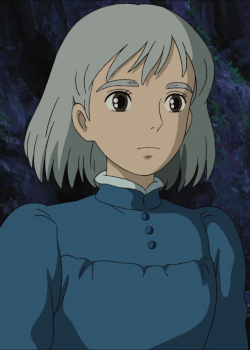
\includegraphics{Images/Characters/sophie}
  \caption{Sohie, movie version}
  \end{figure}
\end{minipage}

\subsubsection*{Relationships}
\begin{itemize}
\item \textbf{Howl}: She is in love with him, her partner. She lives in the flying castle with Howl, Calcifer and their friends.
\item \textbf{Calcifer}: He his her friend and lives with her in the flying castle.
\item \textbf{Justin}: Justin is her friend and the one who makes her meet Howl for the first time.
\item \textbf{Suliman}: She respects Suliman as great magician and due to this fact she trusts her.
\item \textbf{Mizar}: At the beginning she doesn’t know her. She is in conflict with her since she apprehends that Mizar has trapped Howl.
\item \textbf{Belzel}: At the beginning she doesn’t know him. He is her only chance to rescue Howl from the spirits realm.
\end{itemize}

\begin{figure}[H]
  \centering
  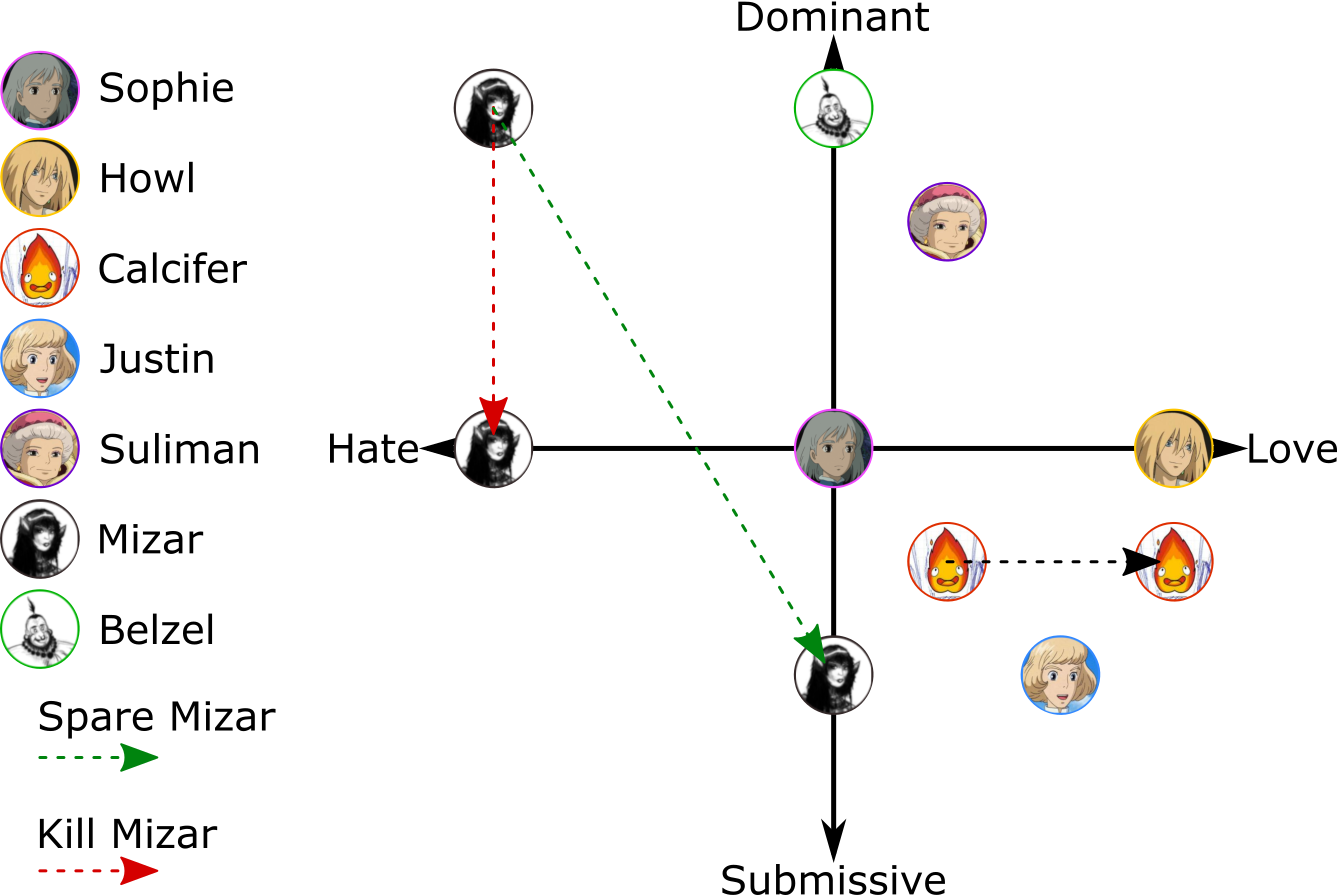
\includegraphics[width=8cm]{Images/Diagrams/Circumplexes/sophieCircumplex}
  \caption{Circumplex of Sophie}
\end{figure}

\begin{figure}[H]
  \centering
  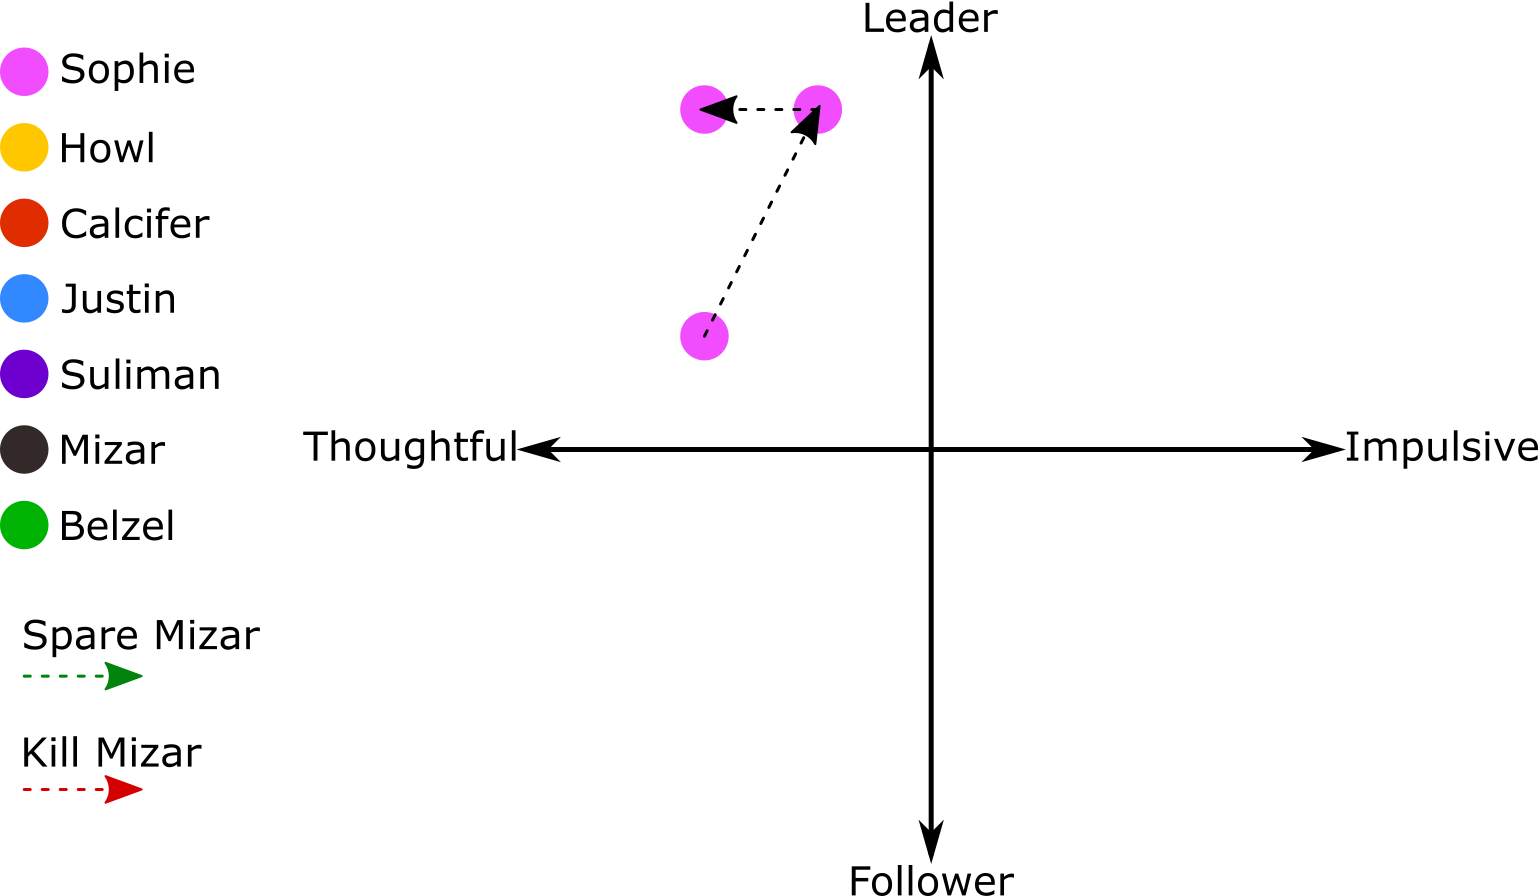
\includegraphics[width=8cm]{Images/Diagrams/Evolutions/sophieEvolution}
  \caption{Evolutions of Sophie}
\end{figure}

\subsection{Description}
Sophie is a brave and altruist girl. She represents the hero of the story who is going to save Howl. She is also optimistic but she always worries about her beloved ones.

Sophie has no combat skills, so she brings with her Calcifer who can protect her from the enemies.

She hasn't lost the passion for hats and occasionally she sews one.

\subsection{Background story}
Before she fell in love with Howl she lived in a small town within the kingdom of Ingary. She is the eldest of two sisters and aimed to become a hatter like her father. After the misadventure of the curse launched by the Wastelands Witch, she has discovered she is a which. Her silver hair is the sign of the passed curse. Her magic powers lets her speak with some objects but she is a novice and she has to learn almost everything about the magic world.
